\section{Data and Knowledge Sources}\label{sec:data}

The system uses five data sources: two for the domain expert's knowledge, one for evaluating it externally, and two for training the vision models that provide case evidence (Table~\ref{tab:datasets}).

\begin{table}[H]
\centering
\caption{Data sources used in the thesis.}
\label{tab:datasets}
\small
\begin{tabularx}{\textwidth}{>{\raggedright\arraybackslash}p{3.4cm} X >{\raggedright\arraybackslash}p{3.8cm}}
\toprule
\textbf{Source} & \textbf{Content} & \textbf{Used for} \\
\midrule
Hematology textbooks \cite{kawthalkar2006,schmaier2012} & 541 PDF pages, 1{,}049 text chunks & RAG knowledge base; source of Q\&A pairs \\
Synthetic hematology Q\&A & 2{,}098 question--answer pairs generated from the chunks & Fine-tuning (1{,}890) and held-out test (208) \\
MedMCQA \cite{pal2022medmcqa} & Medical entrance-exam MCQs; 100-question hematology-related subset & External test of the fine-tuned model \\
TXL-PBC \cite{gan2024txlpbc} & 1{,}260 smear images, 18{,}143 boxes (WBC, RBC, platelet) & Training/testing the cell detector \\
PBC \cite{acevedo2020} & 17{,}092 single-cell images, 8 classes & Training/testing the WBC classifier \\
\bottomrule
\end{tabularx}
\end{table}

\subsection{Hematology textbook corpus}\label{sec:corpus}

The domain knowledge of the expert comes from two hematology textbooks: \emph{Essentials of Haematology} by Kawthalkar \cite{kawthalkar2006} (511 PDF pages) and a 30-page excerpt of the \emph{Concise Guide to Hematology} edited by Schmaier and Lazarus \cite{schmaier2012}. Both books are copyrighted. They were used locally, for non-commercial research, and are not redistributed with the project's code.

Text was extracted page by page with the \code{pypdf} library, whitespace was normalised, and the text was split into chunks of 200 words with an overlap of 40 words between consecutive chunks. The chunk size was chosen so that a chunk fits into the 256-token input limit of the embedding model without being cut. Tables and figures were not parsed and no optical character recognition was performed. The result is 1{,}049 chunks: 996 from the first book and 53 from the second. Each chunk is stored with its source file name and a chunk index (page numbers are not stored).

\subsection{Synthetic question--answer dataset}\label{sec:qa-data}

No public collection of hematology question--answer pairs matched the content of the two textbooks, so a training set was generated from the knowledge base itself (script \code{scripts/build\_finetune\_dataset.py}). For every chunk, an OpenAI GPT model\footnote{The script's default generator is \code{gpt-4o-mini}.} received the passage and the instruction to produce two ``grounded'' question--answer pairs: realistic questions that the passage can answer, with 2--5-sentence answers based \emph{only} on the passage, varying between definitions, mechanisms, differentials, laboratory interpretation and short patient vignettes. Each answer ends with a source line such as ``\textit{Source: essentials\_haematology.pdf.}'' Every training example is stored as a three-message chat (system prompt, question, answer):

\begin{lstlisting}
{"messages": [
  {"role": "system",
   "content": "You are a clinical hematology expert. Always ground answers
               in the provided textbook reference. Use cautious, ..."},
  {"role": "user",
   "content": "What genetic defect is responsible for 40-50% of severe
               cases of haemophilia A?"},
  {"role": "assistant",
   "content": "An inversion in the F VIII gene at intron 22 is responsible
               for 40-50% of cases of severe haemophilia A.
               \n\nSource: essentials_haematology.pdf."}]}
\end{lstlisting}

The generation produced 2{,}098 pairs. Questions are short (13.6 words on average) and answers are concise (about 40 words on average).

\paragraph{Train/test split.} The pairs were split into 90\,\% training and 10\,\% test data \emph{by chunk}: because the generator wrote the two pairs of a chunk consecutively, records $2i$ and $2i{+}1$ were treated as one group, the groups were shuffled with a fixed seed (42), and 10\,\% of the groups were held out. This keeps both questions about the same passage on the same side of the split, so the test questions are about passages the model never saw during fine-tuning. The split contains 1{,}890 training and 208 test pairs (198 and 10 of the test pairs come from the first and the second book, respectively). Both files are saved with the results for reproducibility.

\subsection{External multiple-choice questions (MedMCQA)}

To test whether fine-tuning changes general hematology knowledge --- and not only the ability to reproduce the textbook's answers --- the fine-tuned model was also evaluated on questions that were not derived from the two books. MedMCQA \cite{pal2022medmcqa} contains multiple-choice questions from Indian medical entrance examinations, each with four options and one correct answer. From its validation split, single-answer questions whose topic or question text matched hematology keywords (e.g.\ \emph{haemat-}, \emph{anaemi-}, \emph{leuk-}, \emph{platelet}, \emph{coagul-}, \emph{thalass-}) were selected, and 100 were used. The keyword filter is not perfect: manual inspection shows that roughly a quarter of the selected questions are only loosely related to hematology (for example, questions matched through \emph{hematuria} or \emph{myelopathy}). The subset is therefore described as ``hematology-related'' in the results.

\subsection{Cell detection data: TXL-PBC}

TXL-PBC \cite{gan2024txlpbc} integrates and re-annotates images from four public blood-cell resources (BCCD, BCDD, PBC and Raabin-WBC). It contains 1{,}260 smear images with 18{,}143 bounding boxes in three classes --- white blood cells (WBC), red blood cells (RBC) and platelets --- and is used with its published split of 882 training, 252 validation and 126 test images. The class distribution is dominated by red cells, as in real smears. Annotations are in YOLO format (one text file per image with normalised box coordinates).

\begin{figure}[H]
\centering
\begin{subfigure}[t]{\textwidth}\centering
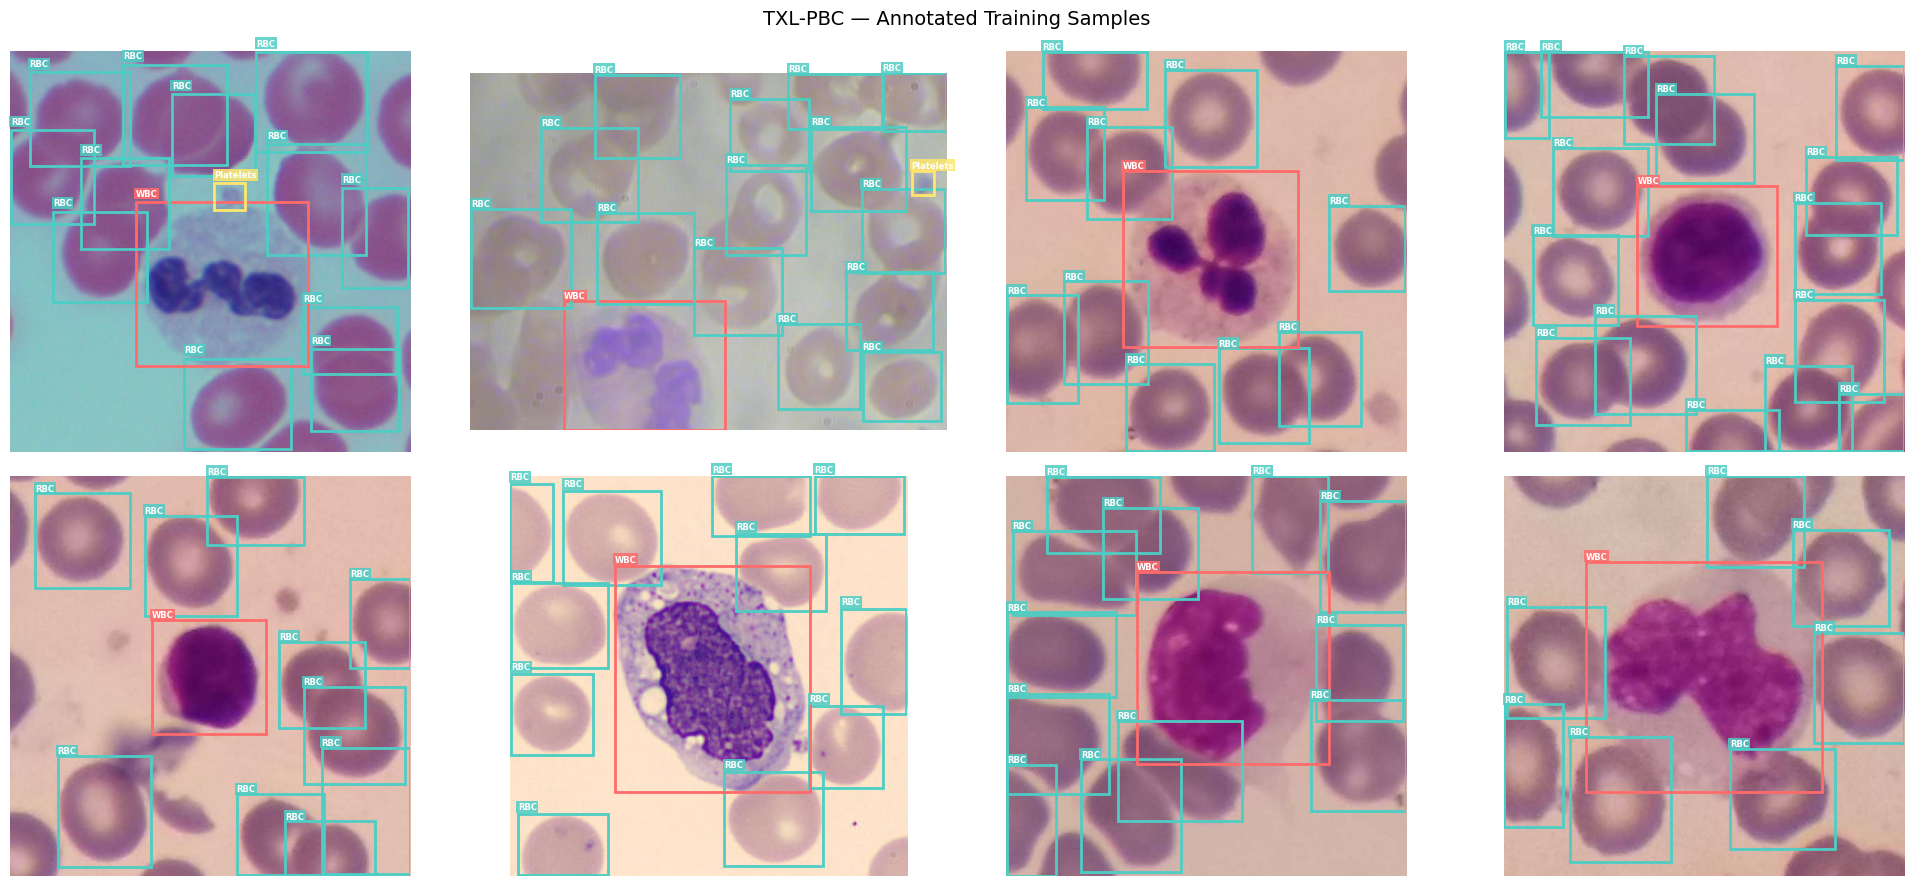
\includegraphics[width=0.95\textwidth]{figures/stage1_embedded_annotated_training_samples.png}
\caption{Annotated training images.}
\end{subfigure}\\[6pt]
\begin{subfigure}[t]{\textwidth}\centering
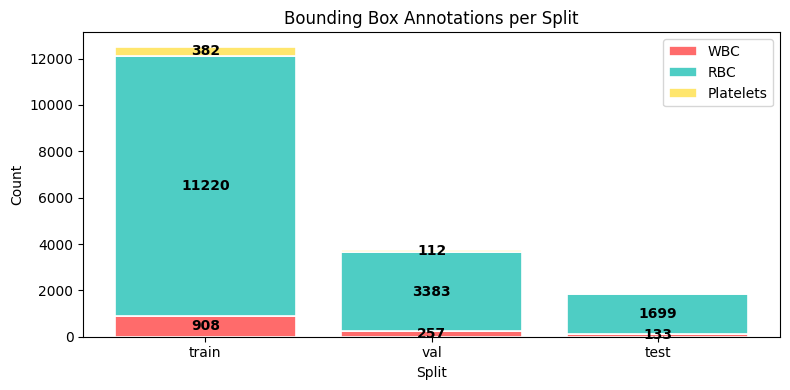
\includegraphics[width=0.62\textwidth]{figures/stage1_embedded_class_distribution_per_split.png}
\caption{Box annotations per split.}
\end{subfigure}
\caption{The TXL-PBC detection dataset: (a) example training images with their WBC, RBC and platelet boxes; (b) number of annotated boxes per class and split, counted from the raw label files (before Ultralytics removed a small number of duplicate labels). Red cells dominate every split.}
\label{fig:txl}
\end{figure}

\subsection{White-cell classification data: PBC}

The PBC dataset of Acevedo \emph{et al.} \cite{acevedo2020} contains 17{,}092 single-cell images of $360 \times 363$ pixels, recorded with a CellaVision DM96 analyser at the Hospital Clínic of Barcelona from individuals without infection, hematological disease or pharmacological treatment. Each image was labelled by clinical pathologists into one of eight classes: \emph{basophil, eosinophil, erythroblast, immature granulocyte (IG), lymphocyte, monocyte, neutrophil} and \emph{platelet}. The classes are moderately imbalanced (about 3{,}300 neutrophils and 1{,}200 basophils). The images were resized to $224 \times 224$ pixels. The final classifier (v2, Section~\ref{sec:method}) uses a class-stratified split into 11{,}963 training, 1{,}710 validation and 3{,}419 test images (70/10/20, seed 42); an earlier run (v1) used an unstratified 80/20 train/test split. Both splits are at image level, not grouped by donor, because the dataset does not identify the donor of each image.

\clearpage
